\documentclass[extendedabs]{bmvc2k}
\usepackage[ruled]{algorithm2e}
\begin{document}

\title{Digital Image Processing HW3}
\addauthor{Hejung Yang}{}{1}
\addinstitution{School of Electrical and Electronic Engineering, 
Yonsei University.}

\maketitle
\vspace{-0.2in}

\section*{problem 1: fft and frequency spectra}

\begin{figure}[h]
    \centering
    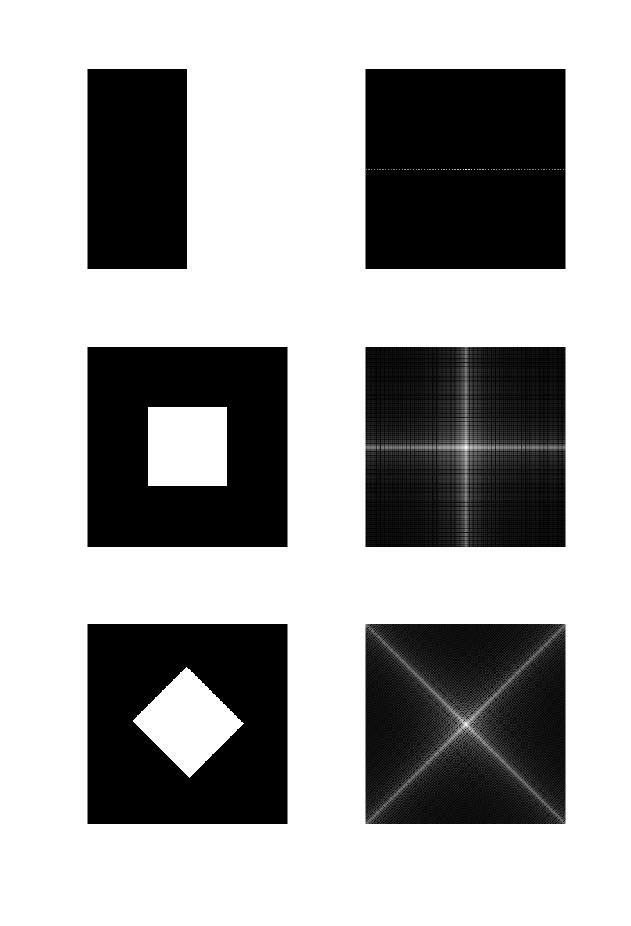
\includegraphics[width=0.7\linewidth]{hw3_1_1}
    \caption{result of prob1.m. each row shows the original image and its magnitude 
    within frequency domain.}
    \label{fig:1}
\end{figure}

In prob1.m, each row contains the spatial domain image and magnitude of its fourier transform output. 
Fourier transform is the transformation which converts spatial(pixel) domain image into complex-valued 
frequency domain image.
Given each image from the first column of \figurename{\ref{fig:1}}, 2-dimensional fft(fast fourier transform)
is applied followed by shifting the zero frequency component to the center of the image.
Extracting magnitude from the complex-valued frequency domain image $\omega$ can be calculated as follows:
\[\omega = \mathcal{F}(image)\]
\[magnitude(\omega) = \sqrt{Real(\omega)^2 + Imag(\omega)^2}\]
Second column of \figurename{\ref{fig:2}} shows each magnitude of given $\omega$. Log scale is applied on
magnitude for better visualization.

At first row, given input image consists of half black and half white dividing the image vertically.
From the fact that the image is constant with respect to the vertial direction and abrupt change occurs
along horizontal direction, especially at the center of the image, it can be expected that the frequency
component is concentrated onto the horizontal line. It can be seen in the magnitude plot that it surely
contains horizontal frequency elements, which stands for vertical edge.

At second row, given input image of white square on the center, it can be seen from
the shifted 2-d fft result that the image contains both horizontal and vertical frequency
component. In third row, it can be visually shown that rotating the spatial domain image also
results the frequency domain image to be rotated accordingly.

\begin{figure}[h]
    \centering
    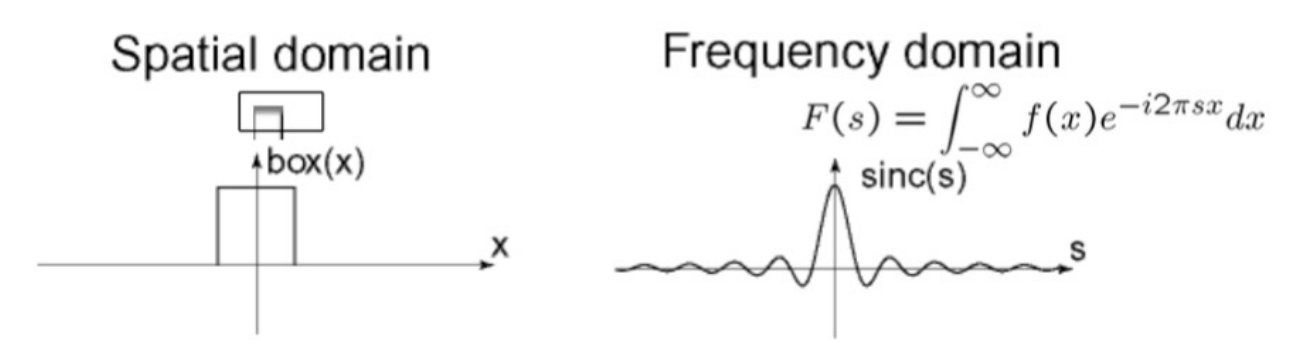
\includegraphics[width=\linewidth]{hw3_1_2}
    \caption{box filter in spatial domain and the corresponding frequency domain function}
    \label{fig:8}
\end{figure}

Another characteristic that can be found in second, third row of \figurename{\ref{fig:1}} is 
that in frequency domain the value fluctuates across the lines. It can be understood from the fact 
that the fourier transform of a box filter is a sinc function (\figurename{\ref{fig:8}}). 
Slicing the second spatial domain image in \figurename{\ref{fig:1}}
across the horizontal/vertical directions generates 1-d box-shaped signal, so it can be expected that 
the resulting frequency domain output of the given image will have fluctuations corresponding to the crossings
of a sinc function. 

\section*{problem 2: phase and magnitude}

\begin{figure}[h]
    \centering
    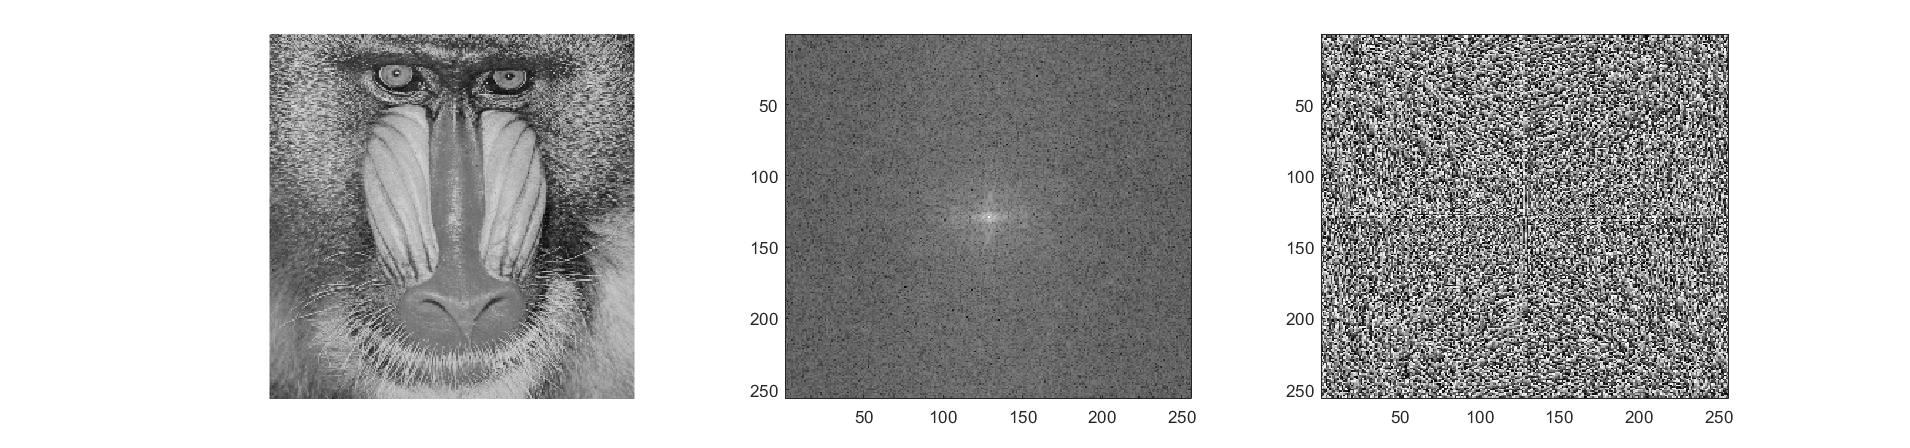
\includegraphics[width=\linewidth]{hw3_2_1}
    \caption{result of hw3\_2.m. leftmost: original image, middle: log-scaled magnitude
    of the given image, rightmost: phase of the image}
    \label{fig:2}
\end{figure}

hw3\_2.m reads image, calculate magnitude/phase after applying 2d fast fourier transform(fft2)
onto the image, shifting the zero frequency component to the center of the image.
As in problem 1, given complex-valued frequency domain image $\omega$, magnitude, phase can be calculated as follows:
\[\omega = \mathcal{F}(image)\]
\[magnitude(\omega) = \sqrt{Real(\omega)^2 + Imag(\omega)^2}\]
\[phase(\omega)) = tan^{-1}\frac{Imag(\omega)}{Real(\omega)}\]
For better visualization, plotted magnitude is log-scaled.
\figurename{\ref{fig:2}} is the magnitude/phase plot of the image.
It can be seen that most of the magnitude is concentrated on the center of the image.
Also, phase image seems to have random values.

\section*{problem 3: phase vs. magnitude}

\begin{figure}[h]
    \centering
    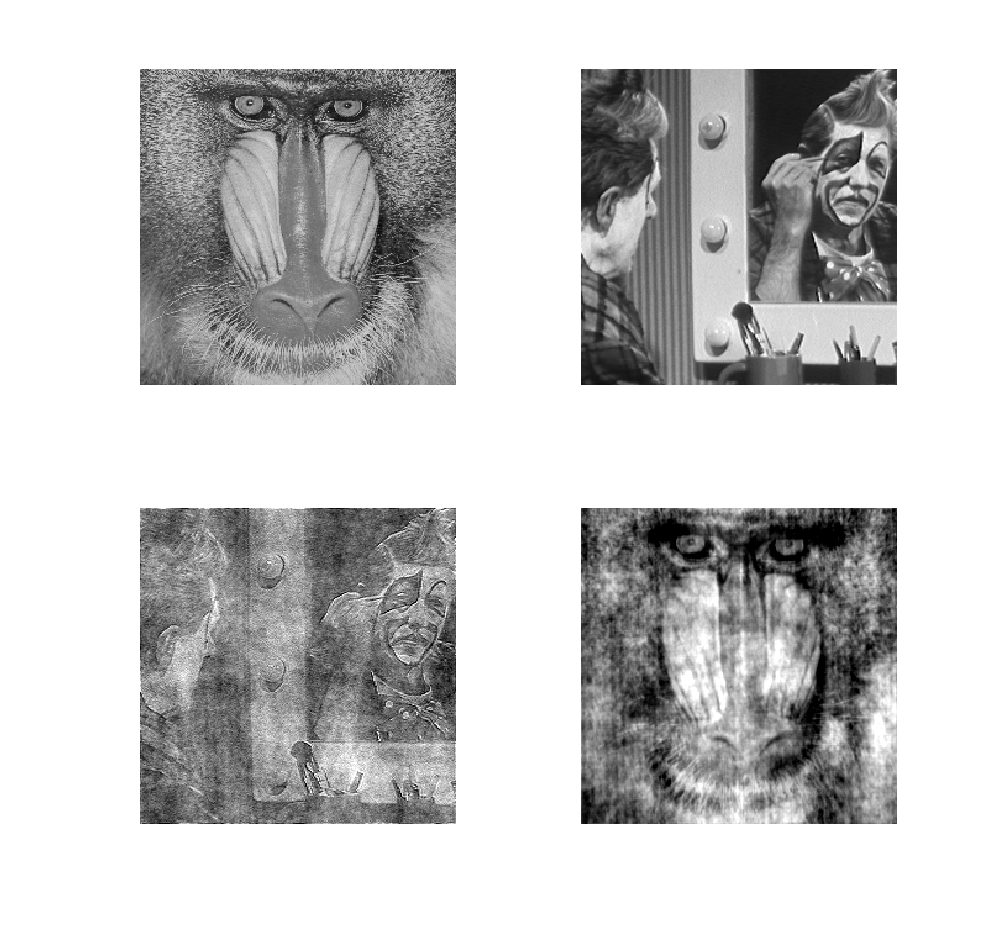
\includegraphics[width=\linewidth]{hw3_3_1}
    \caption{result of hw3\_3.m. top-left: original mandrill image, top-right: original clown image,
    bottom-left: reconstructed image having magnitude of mandrill and phase of clown,
    bottom-right: reconstructed image having magnitude of clown and phase of mandrill}
    \label{fig:3}
\end{figure}

hw3\_3.m reads mandrill and clown image, swaps their phase information and reconstruct the image.
Given magnitude $mag$ and phase $ph$, complex-valued frequency domain image can be calculated as follows:
\[\omega = mag * (cos(ph) + sin(ph) * 1j)\]
\[image = \mathcal{F}^{-1}(\omega)\]

It can be simply seen that the new $\omega$ has magnitude $mag$ and phase $ph$:
\[magnitude(\omega) = \sqrt{Real(\omega)^2 + Imag(\omega)^2}\]
\[= \sqrt{(mag * cos(ph))^2 + (mag * sin(ph))^2}\]
\[= \sqrt{mag^2 * (cos^2(ph) + sin^2(ph))}\]
\[= \sqrt{mag^2} = mag\] 
\[phase(\omega) = tan^{-1}\frac{Imag(\omega)}{Real(\omega)}\]
\[= tan^{-1}\frac{sin(ph)}{cos(ph)}\]
\[= tan^{-1}(tan(ph)) = ph\]

Result of swapping the phase can be found in \figurename{\ref{fig:3}}.
It can be seen that the bottom-left image, consists of mandrill's magnitude and clown's phase,
looks much similar to clown than mandrill. Conversely, bottom-right image which is from clown's
magnitude and mandrill's phase looks like mandrill imge.

\begin{figure}[h]
    \centering
    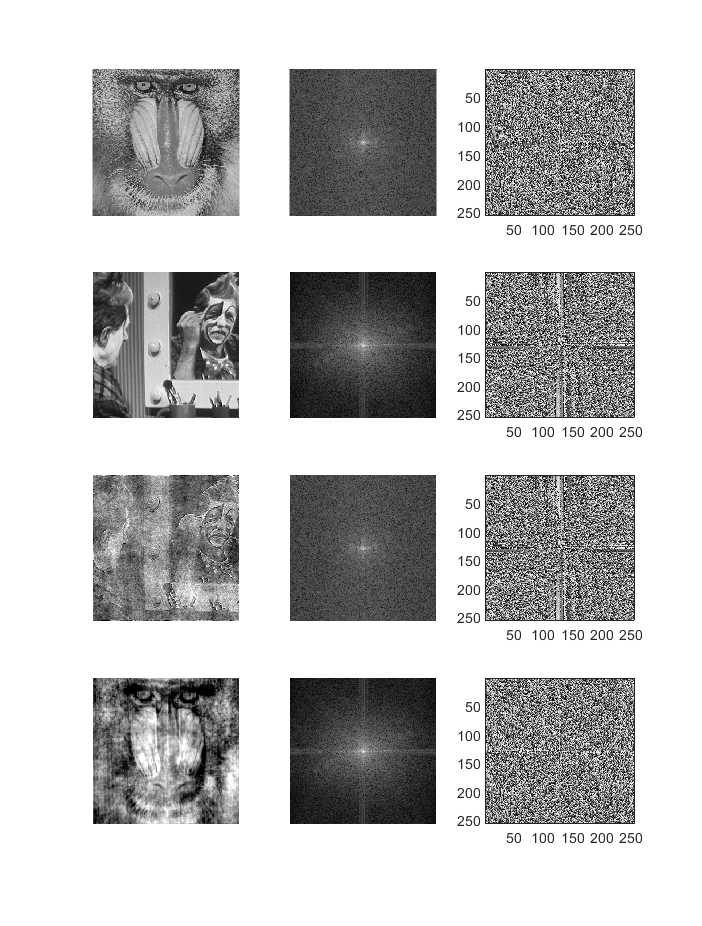
\includegraphics[width=\linewidth]{hw3_3_2}
    \caption{magnitude, phase of images in \figurename{\ref{fig:3}}. Each row stands for
    top-left(mandrill), top-bottom(clown), bottom-left and bottom-right as ordered}
    \label{fig:4}
\end{figure}

\figurename{\ref{fig:4}} shows the magnitude/phase of the original/transformed images. It can
be seen that only the phase information is swapped while having same magnitude.
From the figures, it is shown that phase information is more important than magnitude in terms
of recognizing the object semantic and its structure; magnitude is applied so that the overall
image level is adjusted to the target image. In bottom-left of \figurename{\ref{fig:3}},
though the image is perceived as the clown image, it lost some overall intensity informations compared
to the original clown. Same goes with the bottom-right of \figurename{\ref{fig:3}}. Darkened left 
eye comes from the dark background of the original clown image.

It can be also seen that the details are lost due to the phase-magnitude mismatch. 
Comparing top-right and bottom-left of \figurename{\ref{fig:3}}, detail loss such as stripes on the wall
is found. Even for the mandrill case, detailed fur is hard to recognize compared to the original image.


\section*{problem 4: notch filter}

\begin{figure}[h]
    \centering
    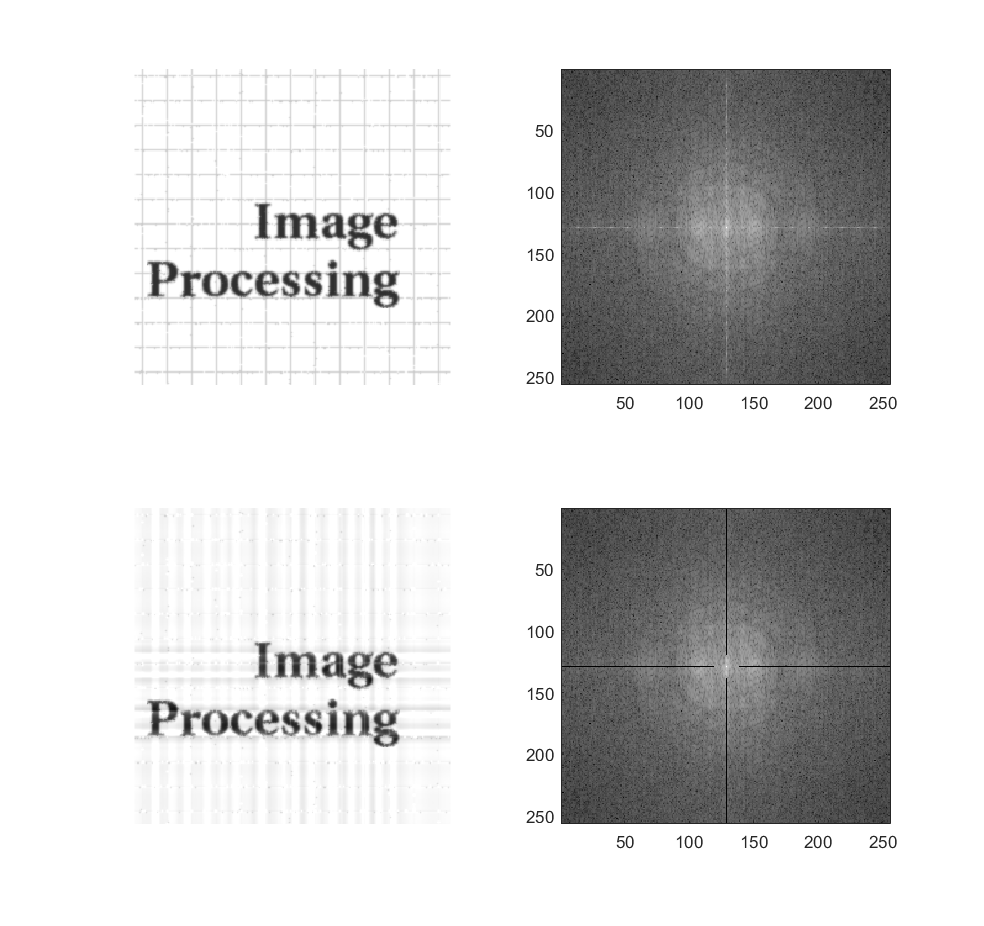
\includegraphics[width=\linewidth]{hw3_4_1}
    \caption{result of hw3\_4.m. top row: original image and its magnitude in frequency 
    domain respectively. bottom row: after applying notch filter onto the frequency domain image
    and its resulting magnitude}
    \label{fig:5}
\end{figure}

hw3\_4.m reads pattern.tif, transform into complex-valued frequency domain, filter out grid pattern
by notch filter and inverse-transform to be able to be seen in spatial domain. 
\figurename{\ref{fig:5}} shows the result of applying notch filter onto the noisy image.
From the magnitude of the original image, it can be seen that there exists outstanding
vertial/horizontal lines which partially represent the grid pattern overlaid onto the original
image. After applying notch filter masking out the vertical/horizontal lines excluding the center,
it can be seen that the grid pattern is smoothed out.

\begin{figure}[h]
    \centering
    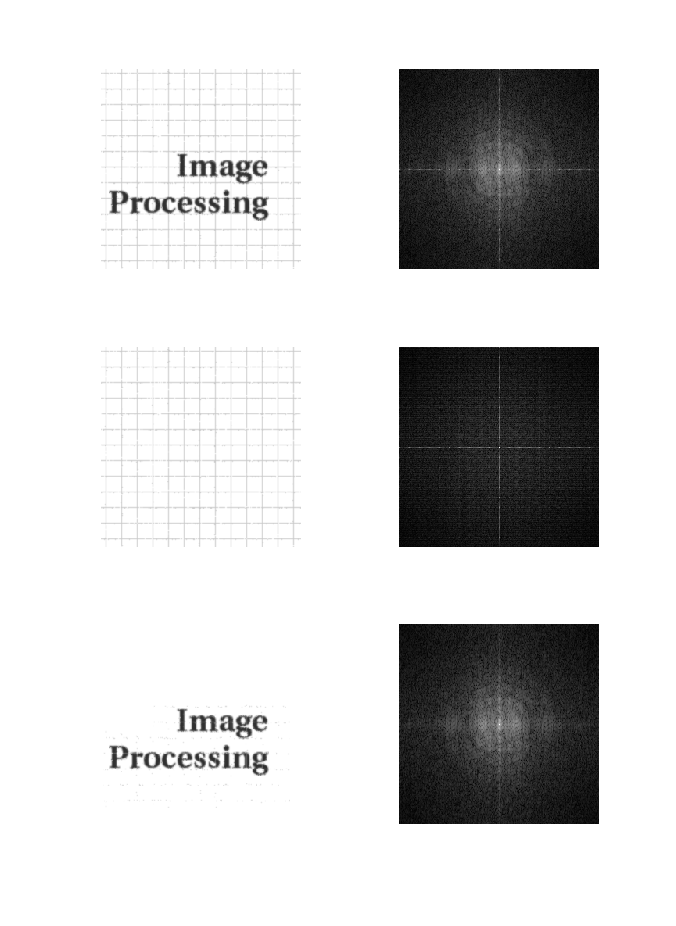
\includegraphics[width=\linewidth]{hw3_4_2}
    \caption{image and magnitude plot for components within the original image. top row: original image
    and its magnitude, middle row: grid-only image with its magnitude, bottom row: after
    subtracting grid from the original image and its magnitude}
    \label{fig:6}
\end{figure}

\figurename{\ref{fig:6}} contains the groundtruth grid pattern and target filtering result.
The groundtruth grid pattern is constructed from pattern.tif using public paint applications.
It can be seen from the middle row of the \figurename{\ref{fig:6}} that the grid pattern mainly consists
of vertical/horizontal elements within the magnitude perspective. Subtracting the image from the
grid pattern generates cleaner image, with having lower intensity on vertical/horizontal lines from
the view of magnitude.

\begin{figure*}[h]
    \centering
    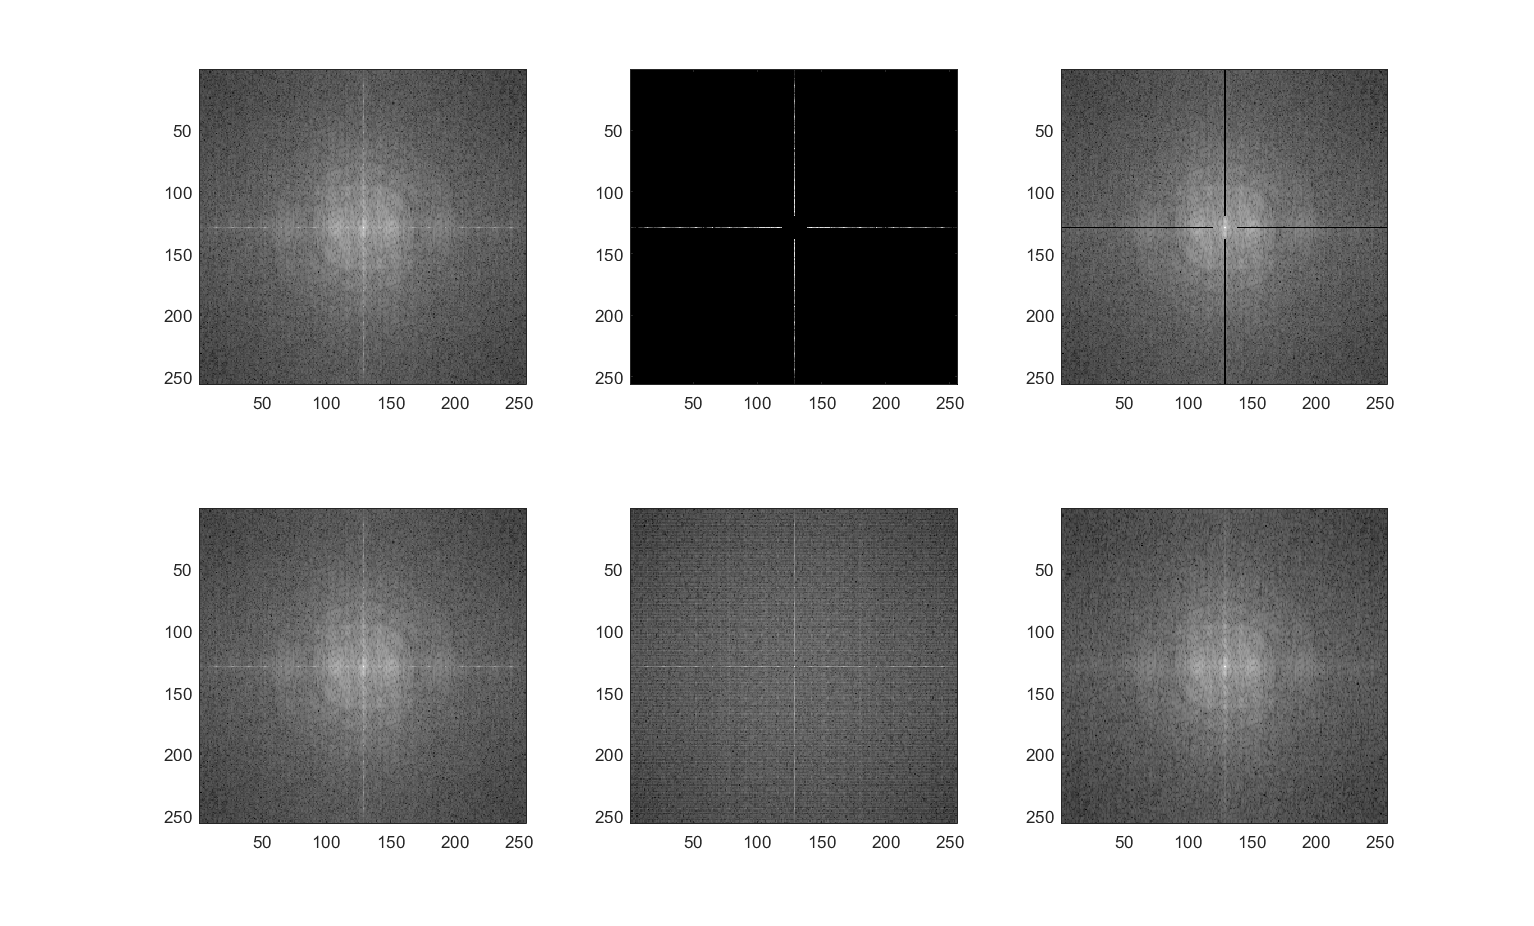
\includegraphics[width=\linewidth]{hw3_4_3}
    \caption{comparison between the notch filter and the groundtruch grid pattern. top row: original image,
    notch filter applied when generating \figurename{\ref{fig:5}} and result after applying the filter 
    respectively. bottom row: same as above except the filter is from the groundtruch grid pattern}
    \label{fig:7}
\end{figure*}

\figurename{\ref{fig:7}} shows the difference between the notch filter which is applied to 
\figurename{\ref{fig:5}} and the groundtruth filter. It can be seen that both the notch
filter and the groundtruth filter contains vertial/horizontal line component within its
magnitude plot but there exists other frequency components contributing to the grid pattern
in the groundtruth plot whereas no other components exist in the notch filter.
Further improvement would be achieved when considering the detailed frequency pattern 
within the grid onto the notch filter.

\end{document}
